\documentclass{article}

\usepackage{graphicx}
\usepackage{tikz}
\usepackage{tikzsymbols}
\usetikzlibrary{calc,patterns,shapes.geometric}
\pagestyle{empty}
\usepackage[margin=0pt]{geometry}
\geometry{papersize={14in,12in}}

\def\centerarc[#1](#2)(#3:#4:#5){\draw[#1] ($(#2)+({#5*cos(#3)},{#5*sin(#3)})$) arc (#3:#4:#5);}

\begin{document}
	\begin{figure}
		\centering
		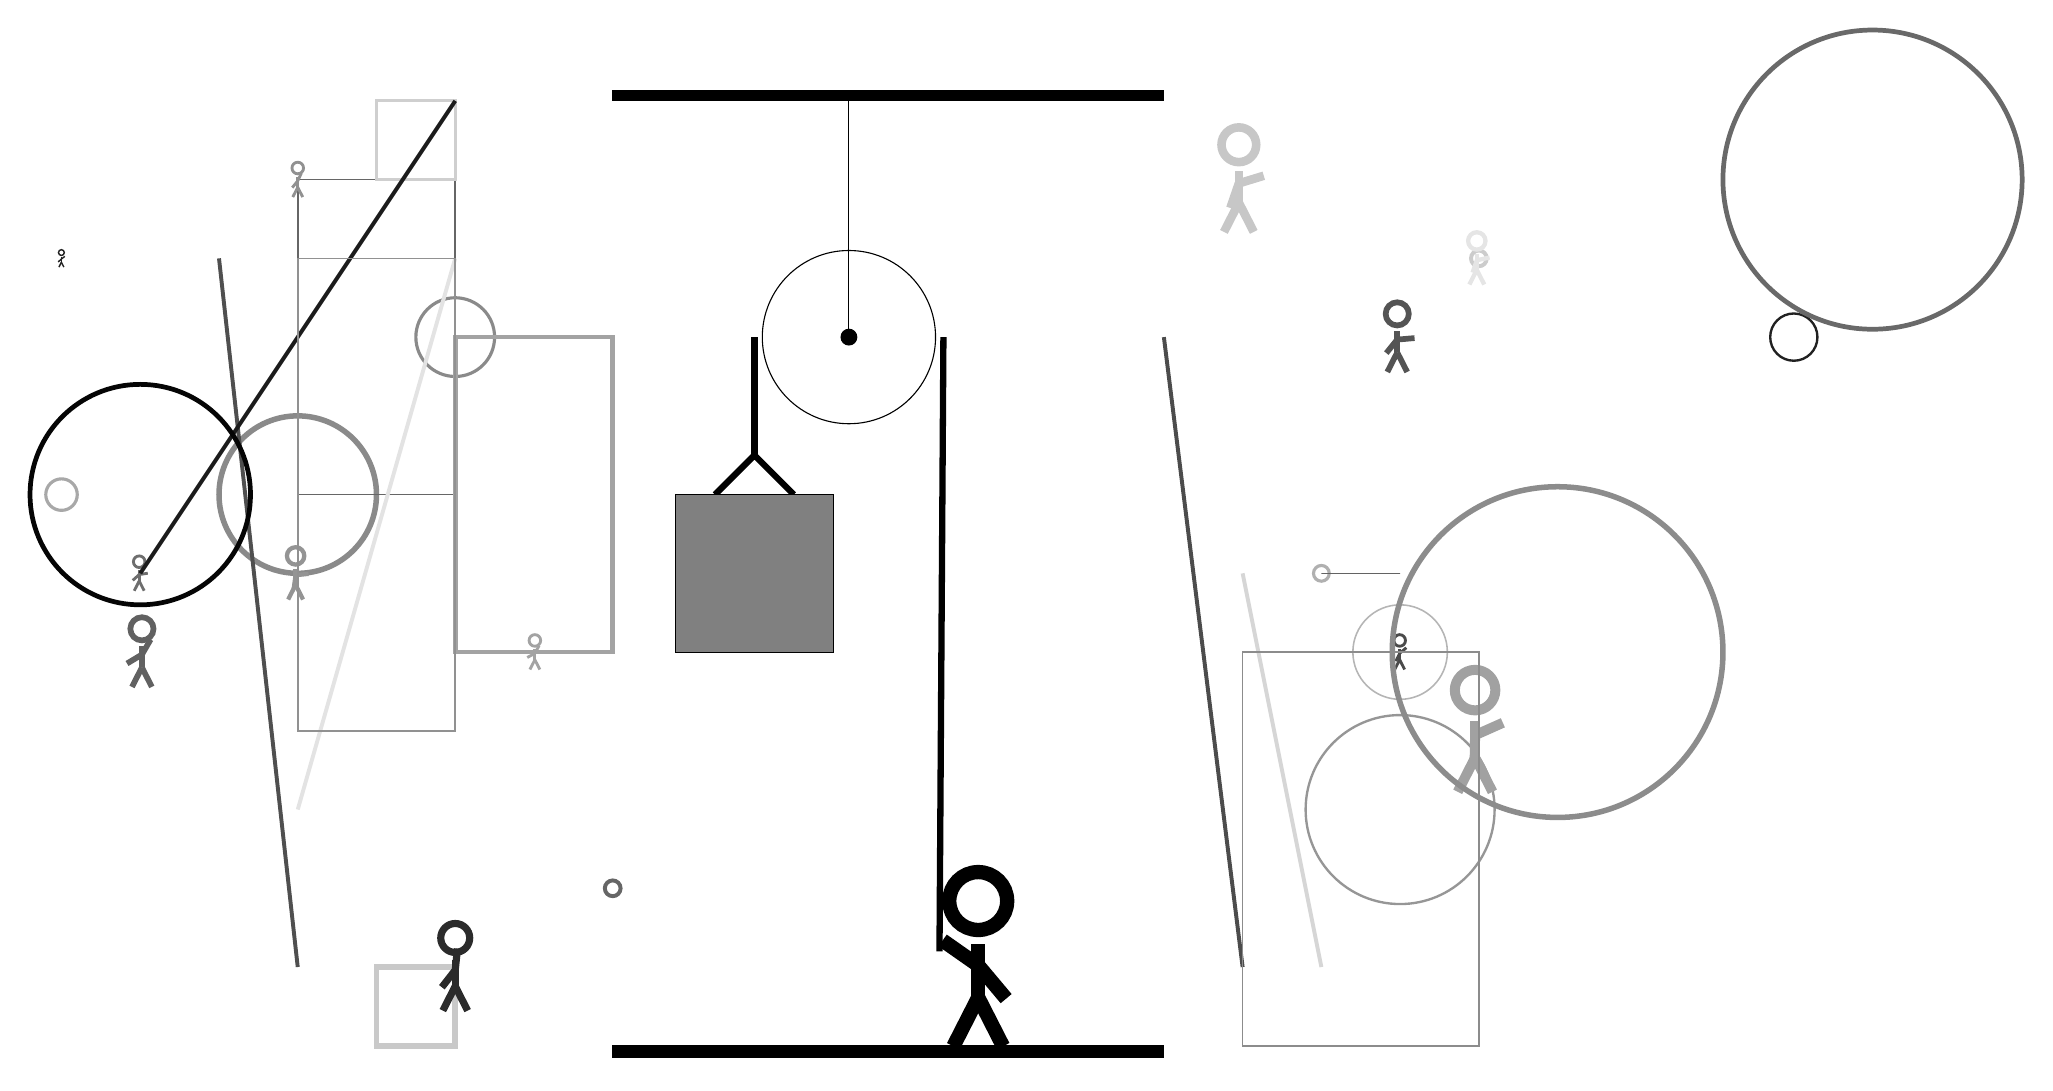
\begin{tikzpicture}
			%%%%% START %%%%%
			
			\draw[fill=black] (-2, 9) rectangle (5, 9.125);
			
			\draw (1, 6) circle (1.1);
			\draw[fill=black] (1, 6) circle (0.1);
			\draw (1, 9) -- (1, 6);
			
			\draw[line width=0.8mm] (-0.7, 4.0) -- (-0.2, 4.5) -- (0.3, 4.0);
			\draw[fill=black!50] (-1.2, 4.0) rectangle (0.8, 2.0);
			
			\draw[line width=0.5mm, color=black!70](5, 6) -- (6, -2);
			
			\node[line width=0.5mm, color=black!22] at (6, 8) {\Strichmaxerl[6][71][17]};
			\draw [line width=0.7mm, color=black!46](-6, 4) circle (1.0);
			\node[line width=0.3mm, color=black!62] at (-8, 2) {\Strichmaxerl[4][31][60]};
			
			\node[line width=0.6mm, color=black!36] at (-3, 2) {\Strichmaxerl[2][29][61]};
			
			\draw[line width=0.2mm, color=black!60] (-4, 8) rectangle (-6, 4);
			
			\draw [line width=0.4mm, color=black!31](7, 3) circle (0.1);
			\draw [line width=0.3mm, color=black!41](8, 0) circle (1.2);
			\draw[line width=0.7mm, color=black!21] (-4, -3) rectangle (-5, -2);
			
			\draw [line width=0.3mm, color=black!87](13, 6) circle (0.3);
			\draw [line width=0.4mm, color=black!46](-4, 6) circle (0.5);
			
			\node[line width=0.3mm, color=black!71] at (8, 2) {\Strichmaxerl[2][64][40]};
			\draw [line width=0.5mm, color=black!20](9, 7) circle (0.1);
			\node[line width=0.7mm, color=black!87] at (-9, 7) {\Strichmaxerl[1][43][37]};
			\node[line width=0.3mm, color=black!83] at (-4, -2) {\Strichmaxerl[5][52][84]};
			\draw [line width=0.4mm, color=black!34](-9, 4) circle (0.2);
			
			\node[line width=0.2mm, color=black!37] at (9, 1) {\Strichmaxerl[7][89][24]};
			\node[line width=0.2mm, color=black!10] at (9, 7) {\Strichmaxerl[3][71][12]};
			\draw [line width=0.2mm, color=black!29](8, 2) circle (0.6);
			
			\draw [line width=0.6mm, color=black!59](14, 8) circle (1.9);
			\draw[line width=0.5mm, color=black!16](7, -2) -- (6, 3);
			\draw[line width=0.2mm, color=black!61] (7, 3) rectangle (8, 3);
			
			\draw[line width=0.6mm, color=black!36] (-4, 2) rectangle (-2, 6);
			\draw[line width=0.4mm, color=black!19] (-4, 8) rectangle (-5, 9);
			\draw [line width=0.5mm, color=black!60](-2, -1) circle (0.1);
			
			\draw [line width=0.7mm, color=black!45](10, 2) circle (2.1);
			\node[line width=0.4mm, color=black!57] at (-8, 3) {\Strichmaxerl[2][42][9]};
			\draw [line width=0.7mm, color=black!53](8, 7) circle (0.0);
			\draw[line width=0.5mm, color=black!69](-7, 7) -- (-6, -2);
			\node[line width=0.2mm, color=black!42] at (-6, 3) {\Strichmaxerl[3][82][6]};
			\node[line width=0.5mm, color=black!43] at (-6, 8) {\Strichmaxerl[2][51][65]};
			
			\draw[line width=0.5mm, color=black!11](-6, 0) -- (-4, 7);
			\node[line width=0.4mm, color=black!67] at (8, 6) {\Strichmaxerl[4][51][5]};
			
			\draw[line width=0.5mm, color=black!89](-4, 9) -- (-8, 3);
			
			\draw[line width=0.2mm, color=black!43] (-4, 7) rectangle (-6, 1);
			\draw[line width=0.2mm, color=black!45] (6, -3) rectangle (9, 2);
			\draw [line width=0.6mm, color=black!98](-8, 4) circle (1.4);
			
			
			\draw[line width=0.8mm] (-0.2, 6) -- (-0.2, 4.5);
			\centerarc[line width=0.8mm](1, 6)(0:180:1.2000000000000002);
			\draw[line width=0.8mm](2.2, 6) -- (2.15, -1.8);
			
			\node at (2.6, -1.9) {\Strichmaxerl[10][-35][-50]};
			
			\draw[fill=black] (-2, -3) rectangle (5, -3.15);
			
			%%%%% END %%%%%
		\end{tikzpicture}
	\end{figure}	
\end{document}